
%----------------------------------------------------------------------------------------
%	PACKAGES AND OTHER DOCUMENT CONFIGURATIONS
%----------------------------------------------------------------------------------------

\documentclass[12pt]{article}

\usepackage{graphicx}
\usepackage{float}
\usepackage{epsfig}
\usepackage{psfrag}
%\usepackage{subfigure}
%\usepackage{subfig}
%\usepackage{tabularx}
\usepackage{subfigmat}
\usepackage{subeqnarray}
\usepackage[colorlinks]{hyperref}
\usepackage{amsmath,amsfonts,amsfonts,amsthm}
\usepackage{xcolor,colortbl}
\usepackage[mathscr]{euscript}
\usepackage{algorithm2e}
\usepackage{siunitx}
\usepackage{rotating}
\usepackage{bm}
\setcounter{secnumdepth}{3}
\usepackage[version=3]{mhchem} 
\usepackage{graphicx}
\usepackage{fancyvrb}
\usepackage[top=1in, bottom=1in, left=1in, right=1in]{geometry}
\graphicspath{{../Figures/}}
\usepackage{color}
\usepackage{pdfpages}
\usepackage{enumitem}
\usepackage{bbm}

\newcommand\alignedbox[2]{
	% Argument #1 = before & if there were no box (lhs)
	% Argument #2 = after & if there were no box (rhs)
	&  % Alignment sign of the line
	{
		\settowidth\dlf{$\displaystyle #1$}  
		% The width of \dlf is the width of the lhs, with a displaystyle font
		\addtolength\dlf{\fboxsep+\fboxrule}  
		% Add to it the distance to the box, and the width of the line of the box
		\hspace{-\dlf}  
		% Move everything dlf units to the left, so that & #1 #2 is aligned under #1 & #2
		\boxed{#1 #2}
		% Put a box around lhs and rhs
	}
}
%----------------------------------------------------------------------------------------
%	ABBREVIATIONS SECTIONS
%----------------------------------------------------------------------------------------
 \newcommand{\dod}{\mathrm{C}_{12}\mathrm{H}_{26}}
 \newcommand{\nit}{\mathrm{N}_{2}}
 \newcommand{\ox}{\mathrm{O}_{2}}
 \newcommand{\wat}{\mathrm{H}_{2}\mathrm{O}}
 \newcommand{\cardiox}{\mathrm{C}\mathrm{O}_{2}}

\begin{document}
%
%%%%%%%%%%%%%%%%%%%%%%%%%%%%%%%%%%%%%%%%%%%%%%%%%%%%%%%%%%%%%%%%%%%%%%
%
\makeatletter
\newcommand\rlarrows{\mathop{\operator@font \rightleftarrows}\nolimits}
\makeatother
%
%%%%%%%%%%%%%%%%%%%%%%%%%%%%%%%%%%%%%%%%%%%%%%%%%%%%%%%%%%%%%%%%%%%%%%
\newenvironment{itemizePacked}{
\begin{itemize}
  \setlength{\itemsep}{1pt}
  \setlength{\parskip}{0pt}
  \setlength{\parsep}{0pt}
}{\end{itemize}}
\newenvironment{enumeratePacked}{
\begin{enumerate}
  \setlength{\itemsep}{5pt}
  \setlength{\parskip}{0pt}
  \setlength{\parsep}{0pt}
}{\end{enumerate}}
% abbreviations %%%%%%%%%%%%%%%%%%%%%%%%%%%%%%%%%%%%%%%%%%%%%%%%%%%%%%
%
%\def\codefont{scriptsize}
\newcommand{\f}[2]{{\frac{#1}{#2}}}
\newcommand{\wt}[1]{{\widetilde{#1}}}
\newcommand{\wh}[1]{{\widehat{#1}}}
\newcommand{\wc}[1]{{\widecheck{#1}}}
\newcommand{\chem}[1]{\ensuremath{\mathrm{#1}}}
\newcommand{\lrangle}[1]{{\langle{#1}\rangle}}
\newcommand{\lrcurl}[1]{{\{{#1}\}}}
\newcommand{\ol}[1]{{\overline{#1}}}
%\newcommand{\ul}[1]{{\underline{#1}}}
\newcommand{\tr}{{\scriptscriptstyle\mathsf T}}
\newcommand{\dd}{{\scriptscriptstyle\Delta}}
\newcommand{\eps}{{\varepsilon}}

\def\RPP{reaction progress parameter}

% boldface-italic font
\newcommand{\bfit}[1]{\textbf{\textit{#1}}}

%
% SOME COLORS %%%%%%%%%%%%%%%%%%%%%%%%%%%%%%%%%%%%%%%%%%%%%%%%%%%%%%%%
%
\newcommand{\colred}[1]{{\color{red} #1}}
\newcommand{\colblue}[1]{{\color{blue} #1}}
\newcommand{\colwhite}[1]{{\color{white} #1}}
\newcommand{\colgreen}[1]{{\color{green} #1}}
\newcommand{\colbrown}[1]{{\color{Brown} #1}}
\newcommand{\colfucsia}[1]{{\color{Fuchsia} #1}}
\newcommand{\colBlue}[1]{{\color{Blue} #1}}
\newcommand{\corrections}[1]{{\color{blue}#1}}
\newcommand{\comment}[1]{{\color{blue}\bf{[#1]}}}
%
% FOR COMBUSTION TEXT %%%%%%%%%%%%%%%%%%%%%%%%%%%%%%%%%%%%%%%%%%%%%%%%
%
\def\chist{\chi_{Z,\up{st}}}
\def\chiq{\chi_{Z,\up{q}}}
\def\chii{\chi_{Z,\up{i}}}
%
% Standard TEX-abbreviations used %%%%%%%%%%%%%%%%%%%%%%%%%%%%%%%%%%%%
%
\def\cldbpage{\clearpage{\pagestyle{empty}\cleardoublepage}}
%
% CALIGRAPHICAL SYMBOLS %%%%%%%%%%%%%%%%%%%%%%%%%%%%%%%%%%%%%%%%%%%%%%
%
\def\cA{{\cal{A}}}
\def\cB{{\cal{B}}}
\def\cC{{\cal{C}}}
\def\cO{{\cal{O}}}
\def\cD{{\cal{D}}}
\def\cE{{\cal{E}}}
\def\cF{{\cal{F}}}
\def\cH{{\cal{H}}}
\def\cJ{{\cal{J}}}
\def\cG{{\cal{G}}}
\def\cN{{\cal{N}}}
\def\cL{{\cal{L}}}
\def\cS{{\cal{S}}}
\def\cT{{\cal{T}}}
\def\cU{{\cal{U}}}
\def\cC{{\cal{C}}} 
\def\cZ{{\cal{Z}}}
\def\cM{{\cal{M}}}
\def\cP{{\cal{P}}}
\def\cR{{\cal{R}}}
\def\cV{{\cal{V}}}
\def\cQ{{\cal{Q}}}
%
% NEW FUNCTION NAMES %%%%%%%%%%%%%%%%%%%%%%%%%%%%%%%%%%%%%%%%%%%%%%%%%
%
\def\erf{{\rm{erf}}}
%
% TEXT FONT DEFINITIONS %%%%%%%%%%%%%%%%%%%%%%%%%%%%%%%%%%%%%%%%%%%%%%
%
\def\up{\textup}
\def\p{\partial}
\def\d{\textup d}
\def\D{\displaystyle}
%\def\S{\scriptsize}
\def\OmFint{\iiint\limits_{\OmF}}
\def\OmF{{\Omega_{\cal F}}}
\def\OmA{{\Omega_{\cal A}}}
\def\e{\textup{e}}
\def\i{\textup{i}}
\def\REFUP{\rm{ref}}
\def\REF{_{\REFUP}}
%
% DIMENSIONLESS QUANTITIES %%%%%%%%%%%%%%%%%%%%%%%%%%%%%%%%%%%%%%%%%%%
%
%\def\Re{{\rm{Re}}}
\def\Fr{{\rm{Fr}}}
\def\M{{\rm{M}}}
\def\Ce{{\rm{Ce}}}
\def\Re{{\rm{Re}}}
\def\Rd{{\rm{Rd}}}
\def\Le{{\rm{Le}}}
\def\Da{{\rm{Da}}}
\def\Ka{{\rm{Ka}}}
\def\Nu{{\rm{Nu}}}
\def\Sc{{\rm{Sc}}}
\def\Ri{{\rm{Ri}}}
\def\Ec{{\rm{Ec}}}
\def\Tu{{\rm{Tu}}}
\def\St{{\rm{St}}}
\def\Mi{{\rm{Mi}}}
\def\Ra{{\rm{Ra}}}
\def\Ze{{\rm{Ze}}}
%
% FOR LATEX %%%%%%%%%%%%%%%%%%%%%%%%%%%%%%%%%%%%%%%%%%%%%%%%%%%%%%%%%%
%
 \def\avec{{\mbox{\boldmath$a$}}}
 \def\bvec{{\mbox{\boldmath$b$}}}
 \def\Bvec{{\mbox{\boldmath$B$}}}
 \def\cvec{{\mbox{\boldmath$c$}}}
 \def\dvec{{\mbox{\boldmath$d$}}}
 \def\evec{{\mbox{\boldmath$e$}}}
 \def\Fvec{{\mbox{\boldmath$F$}}}
 \def\Nvec{{\mbox{\boldmath$N$}}}
 \def\fvec{{\mbox{\boldmath$f$}}}
 \def\gvec{{\mbox{\boldmath$g$}}}
 \def\hvec{{\mbox{\boldmath$h$}}}
 \def\ivec{{\mbox{\boldmath$i$}}}
 \def\jvec{{\mbox{\boldmath$j$}}}
 \def\kvec{{\mbox{\boldmath$k$}}}
 \def\pvec{{\mbox{\boldmath$p$}}}
 \def\Pvec{{\mbox{\boldmath$P$}}}
 \def\uvec{{\mbox{\boldmath$u$}}}
 \def\Uvec{{\mbox{\boldmath$U$}}}
 \def\nvec{{\mbox{\boldmath$n$}}}
 \def\tvec{{\mbox{\boldmath$t$}}}
 \def\Rvec{{\mbox{\boldmath$R$}}}
 \def\rvec{{\mbox{\boldmath$r$}}}
 \def\svec{{\mbox{\boldmath$s$}}}
 \def\Svec{{\mbox{\boldmath$S$}}}
 \def\xvec{{\mbox{\boldmath$x$}}}
 \def\vvec{{\mbox{\boldmath$v$}}}
 \def\wvec{{\mbox{\boldmath$w$}}}
 \def\yvec{{\mbox{\boldmath$y$}}}
 \def\mvec{{\mbox{\boldmath$m$}}}
 \def\Xvec{{\mbox{\boldmath$X$}}}
 \def\qvec{{\mbox{\boldmath$q$}}}
 \def\0vec{{\mbox{\boldmath$0$}}}
 \def\xivec{{\mbox{\boldmath$\xi$}}}
 \def\rhovec{{\mbox{\boldmath$\rho$}}}
 \def\wpvec{{\boldsymbol{\wp}}}
 \def\psivec{{\mbox{\boldmath$\psi$}}}
 \def\epsvec{{\mbox{\boldmath$\epsilon$}}}
 \def\phivec{{\mbox{\boldmath$\phi$}}}
 \def\varphivec{{\mbox{\boldmath$\varphi$}}}
 \def\zetavec{{\mbox{\boldmath$\zeta$}}}
 \def\kappavec{{\mbox{\boldmath$\kappa$}}}
 \def\varkappavec{{\pmb{\varkappa}}}
 \def\etavec{{\mbox{\boldmath$\eta$}}}
 \def\Psivec{{\boldsymbol{\Psi}}}
 \def\Phivec{{\boldsymbol{\Phi}}}
 \def\Wvec{{\boldsymbol{W}}}
 \def\Yvec{{\mbox{\boldmath$Y$}}}
 \def\Vvec{{\mbox{\boldmath$V$}}}
 \def\cLvec{{\boldsymbol{\cal{L}}}}
 \def\cMvec{{\boldsymbol{\cal{M}}}}
 \def\omegavec{{\mbox{\boldmath$\omega$}}}
 \def\Omegavec{{\mbox{\boldmath$\Omega$}}}
 \def\sigmavec{{\boldsymbol{\sigma}}}
 \def\Amat{{\underline{\underline{{A}}}}}
 \def\Bmat{{\underline{\underline{{B}}}}}
 \def\Phimat{{\underline{\underline{{\Phi}}}}}
 \def\taumat{{\underline{\underline{{\tau}}}}}
 \def\sigmamat{{\underline{\underline{{\sigma}}}}}
 \def\Cmat{{\underline{\underline{{C}}}}}
 \def\Imat{{\underline{\underline{{I}}}}}
 \def\Jmat{{\underline{\underline{{J}}}}}
 \def\Smat{{\underline{\underline{{S}}}}}
 \def\Rmat{{\underline{\underline{{R}}}}}
 \def\Tmat{{\underline{\underline{{T}}}}}
 \def\Emat{{\underline{\underline{{E}}}}}
 \def\tmat{{\underline{\underline{{t}}}}}

 \def\alphavec{{\boldsymbol{\alpha}}}
 \def\betavec{{\boldsymbol{\beta}}}
 \def\tauvec{{\boldsymbol{\tau}}}
 \def\thetavec{{\boldsymbol{\theta}}}
 \def\lambdavec{{\mbox{\boldmath$\lambda$}}}
 \def\cTmat{{\underline{\underline{{\cal{T}}}}}}
 \def\cLmat{{\underline{\underline{{\cal{L}}}}}}
 \def\cMmat{{\underline{\underline{{\cal{M}}}}}}
 \def\kappamat{{\underline{\underline{{\kappa}}}}}
%
% Grad, Div, ... %%%%%%%%%%%%%%%%%%%%%%%%%%%%%%%%%%%%%%%%%%%%%%%%%%%%%
%
\def\Grad{\nabla}
\def\Div{\nabla \cdot}
\def\Lap{\nabla^2}
%

\begin{titlepage}

\newcommand{\ddz}[1]{\frac{\mathrm{d} #1}{\mathrm{d} z}}
\newcommand{\HRule}{\rule{\linewidth}{0.5mm}} % Defines a new command for the horizontal lines, change thickness here

\center % Center everything on the page
 

 
%----------------------------------------------------------------------------------------
%	HEADING SECTIONS
%----------------------------------------------------------------------------------------


%\textsc{\Large STANFORD UNIVERSITY}\\[1.5cm] % Name of your university/college

%----------------------------------------------------------------------------------------
%	TITLE SECTION
%----------------------------------------------------------------------------------------

\HRule \\[1 cm]
{ \huge \bfseries Final Project Reference Solutions}\\[0.4cm] % Title of your document
\HRule \\[2cm]
 
%----------------------------------------------------------------------------------------
%	AUTHOR SECTION
%----------------------------------------------------------------------------------------

\Large  \textsc{Matthias Ihme}\\[2cm] % Your name
\textsc{\large ME 257/357: Propulsion System and Gas-Turbine Analysis}\\[2cm] % Major heading such as course name

%----------------------------------------------------------------------------------------
%	LOGO SECTION
%----------------------------------------------------------------------------------------

\includegraphics[width=50mm]{stanford_seal.png}\\[2cm] % Include a department/university logo - this will require the graphicx package
%----------------------------------------------------------------------------------------
%----------------------------------------------------------------------------------------
%	DATE SECTION
%----------------------------------------------------------------------------------------
{\large Spring 2018}%\\[3cm] % Date, change the \today to a set date if you want to be precise

\vfill % Fill the rest of the page with whitespace

\end{titlepage}

%----------------------------------------------------------------------------------------
%	BODY SECTION
%----------------------------------------------------------------------------------------

%%%%%%%%%%%%%%%%%%%%%%%%%%%%%%%%%%%%%%%%%%%%%%%%%%%%%%%%%%%%%%%%%%%%%%%%%%%%%%%%  
\section{Part 1 Turbine Stator-Rotor Analysis [20 pts]}
\begin{itemize}
	\item[a)[3 pts]]
	The velocity triangles are shown in Figure~\ref{fig:stator_rotor}.
	\begin{figure}[H]
		\centering
		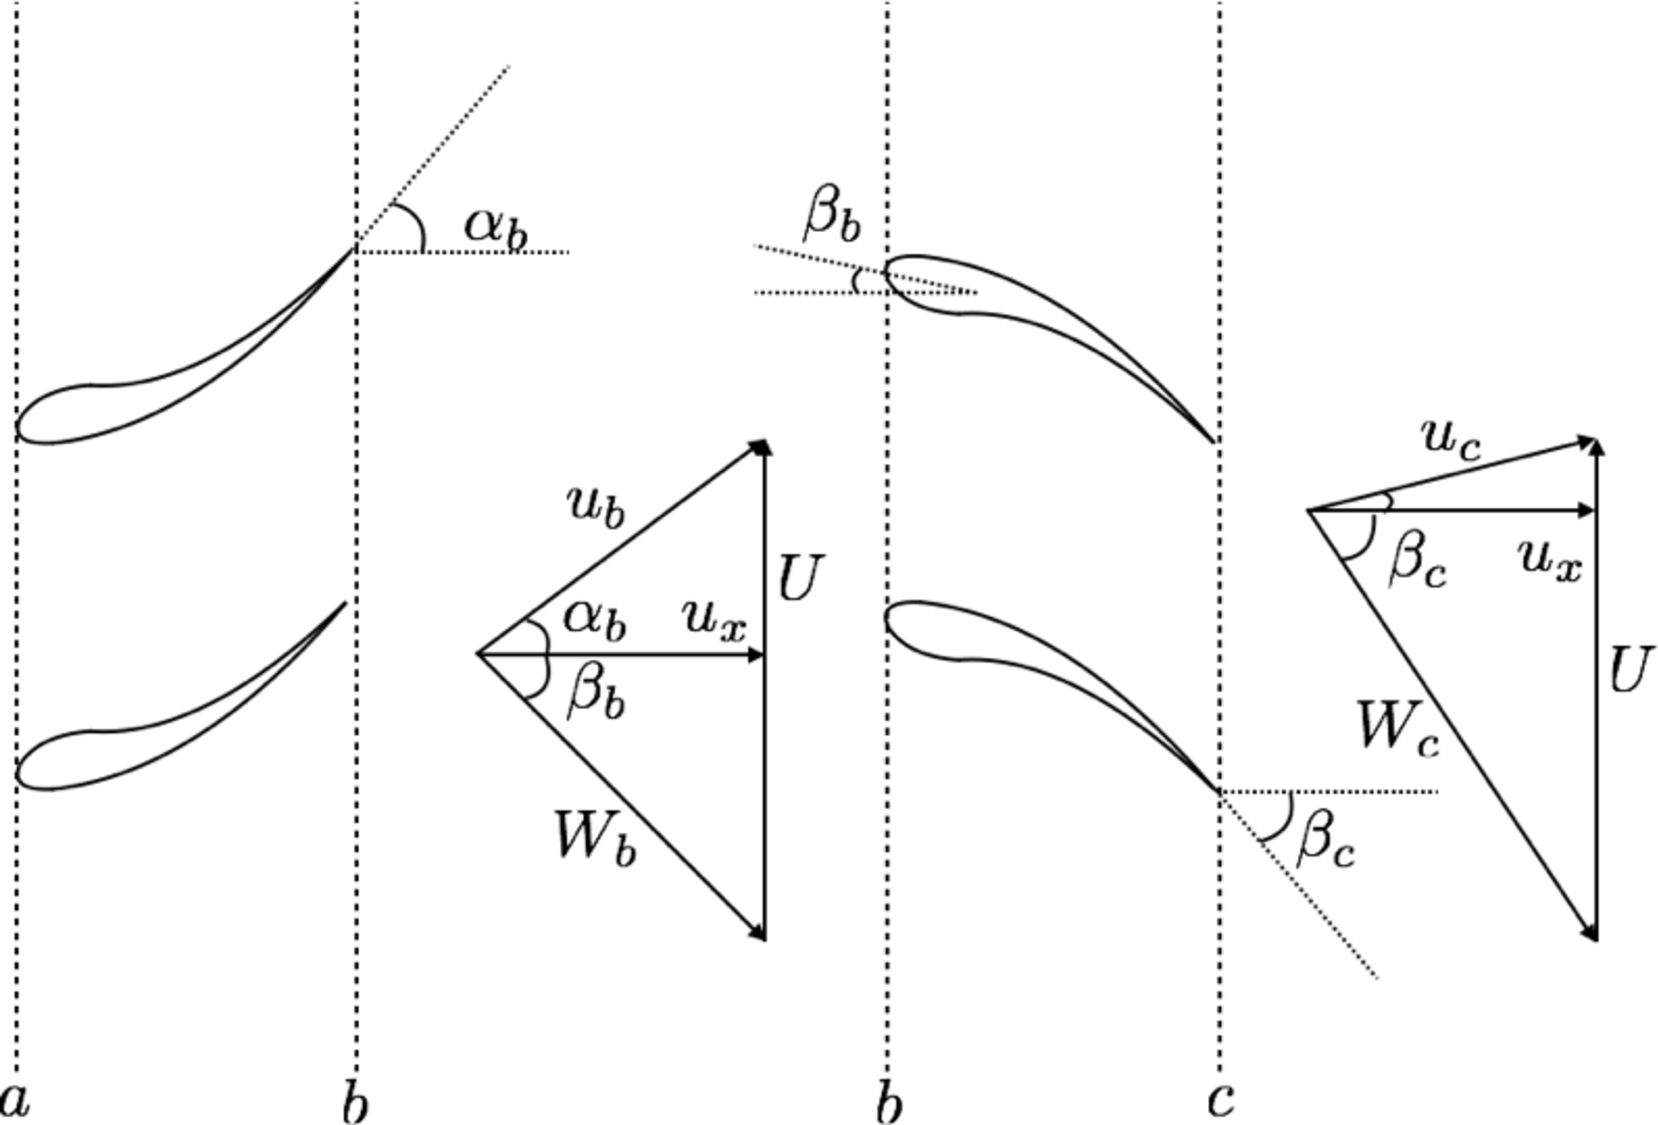
\includegraphics[width=0.6\textwidth]{stator_rotor}
		\caption{Turbine stage stator-rotor combination and velocity triangles.}
		\label{fig:stator_rotor}
	\end{figure}
	
	\item[b)[5 pts]]
	Note that $u_{\theta,b} = u_x \tan \alpha_b$ and $u_{\theta,c} = U - u_x \tan \beta_c$, the work extracted for a single stage is:
	\begin{align}
		\Delta h_0 &= h_{0a} - h_{0c} \nonumber \\
				   &= U\delta u_{\theta} \nonumber \\
				   &= U \left[ u_x \left(\tan \alpha_b + \tan \beta_c\right) - U\right] \nonumber \\
				   &= U^2 \left[ \frac{u_x}{U} \left(\tan \alpha_b + \tan \beta_c\right) - 1\right].
	\end{align}
	Also note that $h_{0a} - h_{0c} = C_p\left(T_{0a}-T_{0c}\right)$, then
	\begin{align}
		1 - \frac{T_{0c}}{T_{0a}} &= \frac{U}{C_p T_{0a}} \left[ u_x \left(\tan \alpha_b + \tan \beta_c\right) - U\right] \nonumber \\
								  &= \frac{U}{\frac{\gamma}{\gamma - 1}R T_{0a}} \left[ u_x \left(\tan \alpha_b + \tan \beta_c\right) - U\right] \nonumber \\
								  &= \left(\gamma - 1\right)\frac{U}{\gamma R T_{0a}} \left[ u_x \left(\tan \alpha_b + \tan \beta_c\right) - U\right] \nonumber \\
								  &= \left(\gamma - 1\right)\frac{U}{\sqrt{\gamma R T_{0a}}} \left[ \frac{u_x}{\sqrt{\gamma R T_{0a}}} \left(\tan \alpha_b + \tan \beta_c\right) - \frac{U}{\sqrt{\gamma R T_{0a}}}\right].
	\end{align}
	
	\item[c)[5 pts]]
	Stage efficiency for single turbine stage is:
	\begin{equation}
		\eta_\text{st} = \frac{h_{0a} - h_{0c}}{h_{0a} - h_{0cs}} = \frac{\frac{T_{0cs}}{T_{0a}}-1}{\frac{T_{0c}}{T_{0a}}-1}.
	\end{equation}
	Hence we have:
	\begin{equation}
		\frac{T_{0cs}}{T_{0a}} = 1 + \frac{1}{\eta_\text{st}}\left( \frac{T_{0c}}{T_{0a}}-1\right).
	\end{equation}
	From the isentropic relationship, we have:
	\begin{equation}
		\frac{p_{0c}}{p_{0a}} = \left[1 + \frac{1}{\eta_\text{st}}\left( \frac{T_{0c}}{T_{0a}}-1\right)\right]^{\frac{\gamma}{\gamma - 1}}.
	\end{equation}
	
	For an $n$-stage turbine, across the $k^\text{th}$ stage, note that $C_p \left(T_{0k} - T_{0,k-1}\right) = -U\Delta u_\theta$ hence $T_{0k} = T_{01} - \left[\left(k - 1 \right)U\Delta u_\theta \right]/C_p$, we have:
	\begin{align}
		\frac{T_{0,k+1,s}}{T_{0k}} &= 1 + \frac{1}{\eta_\text{st}}\left( \frac{T_{0c}}{T_{0a}}-1\right) \nonumber \\
								   &= 1 - \frac{1}{\eta_\text{st}}\frac{U\Delta u_\theta}{C_p T_{0k}} \nonumber \\
								   &= 1 - \frac{1}{\eta_\text{st}}\frac{U\Delta u_\theta}{C_p T_{01}\left(1 - (k-1)\frac{U\Delta u_\theta}{C_p T_{01}}\right)}.
	\end{align}
	Therefore the pressure ratio for the $n$-stage turbine is:
	\begin{align}
		\frac{p_{0,n+1}}{p_{01}} &= \left( \frac{T_{0,n+1,s}}{T_{0n}}\right)^{\frac{\gamma}{\gamma - 1}} \nonumber \\
								 &= \left\{\prod_{k = 1}^{n} \left[1 - \frac{1}{\eta_\text{st}}\frac{U\Delta u_\theta}{C_p T_{01}\left(1 - (k-1)\frac{U\Delta u_\theta}{C_p T_{01}}\right)}\right]\right\}^{\frac{\gamma}{\gamma - 1}}
	\end{align}
	The temperature ratio is:
	\begin{equation}
		\frac{T_{0,n+1}}{T_{01}} = 1 - \left[\left(k - 1 \right)U\Delta u_\theta \right]/{C_p T_{01}}.
	\end{equation}
	The $n$-stage turbine efficiency is then:
	\begin{align}
		\eta_\text{T} &= \frac{1 - \frac{T_{0,n+1}}{T_{01}}}{1 - \frac{T_{0,n+1,s}}{T_{01}}} \nonumber \\
					  &= \frac{\left[\left(k - 1 \right)U\Delta u_\theta \right]/{C_p T_{01}}}{1 - \prod_{k = 1}^{n} \left[1 - \frac{1}{\eta_\text{st}}\frac{U\Delta u_\theta}{C_p T_{01}\left(1 - (k-1)\frac{U\Delta u_\theta}{C_p T_{01}}\right)}\right]}.
	\end{align}
	
	\item[d)[7 pts]]
	See solution code.
	
\end{itemize}
%%%%%%%%%%%%%%%%%%%%%%%%%%%%%%%%%%%%%%%%%%%%%%%%%%%%%%%%%%%%%%%%%%%%%%%%%%%%%%%%  
\section{Part 2 Turbine Design [30 pts]}
\begin{itemize}
	\item[e)[5 pts]]
	The mechanical constraint is that the compressor and the turbine has the same angular velocity. From the compressor:
	\begin{equation}
		\omega = \frac{U_c}{\overline{r}_c} = \frac{310}{0.115} = 2695.65\text{ s}^{-1}.
	\end{equation}
	Then the turbine velocity at the pitchline is:
	\begin{equation}
		U_t = \omega \overline{r}_t = 2195.65\text{ s}^{-1}\times 0.08 = 215.65\text{m/s}.
	\end{equation}
	
	\item[f)[5 pts]]
	Ignoring the fuel-air ratio when using mass balance between HPC and HPT, we have $\dot{m}_t \approx \dot{m}_\text{core}=2.825$ kg/s. When choked at the turbine inlet, i.e. $M_4 = 1$, $f(M_4=1)=A_4/A^*_4=1$. Note that $P_{04} = P_{03} = \pi_c P_{02.5}=12P_{02.5} = 988.8kPa$, using the mass flow rate equation provided, $A_4$ can be computed as:
	\begin{equation}
		A_4 = \dot{m}_t \frac{\sqrt{\gamma R T_{04}}}{P_{04}f(M_4)}\frac{1}{\gamma}\left( \frac{\gamma + 1}{2}\right)^{\frac{\gamma + 1}{2\left( \gamma - 1\right)}} = 2.827\times 10^{-3}\text{ m}^2.
	\end{equation}
	From the geometry, $A_4 = \pi \left(r^2_\text{tip} - r^2_\text{hub}\right)$, $\overline{r} = 0.5\left(r_\text{tip} + r_\text{hub}\right)$. Therefore, $r_\text{tip} = 0.082812$ m and $r_\text{hub} = 0.077188$ m, the hub-to-tip ratio is $r_\text{hub}/r_\text{tip} = 0.932$.
	
	Besides $\alpha_b$ and $\beta_c$, we also need to know the axial velocity $u_x$, the stage efficiency, and the number of stages in the turbine.
	
	\item[g)[5 pts]]
	From $h_0 = h + (1/2) u^2$, $h = C_p T$, $C_p = \gamma R/(\gamma - 1)$, $a = \sqrt{\gamma R T}$, and $M = u / a$, we have:
	\begin{equation}
		\frac{T_0}{T} = 1 + \left(\frac{\gamma - 1}{2}\right) M^2.
	\end{equation}
	Therefore we have:
	\begin{equation}
		u = M \left[\gamma R T_0\left(1 + \left(\frac{\gamma - 1}{2}\right) M^2\right)^{-1}\right]^{1/2}.
		\label{eq:u_M}
	\end{equation}
	
	\item[h)[5 pts]]
	Desired work map is shown in Figure~\ref{fig:p2h}.
	\begin{figure}[H]
		\centering
		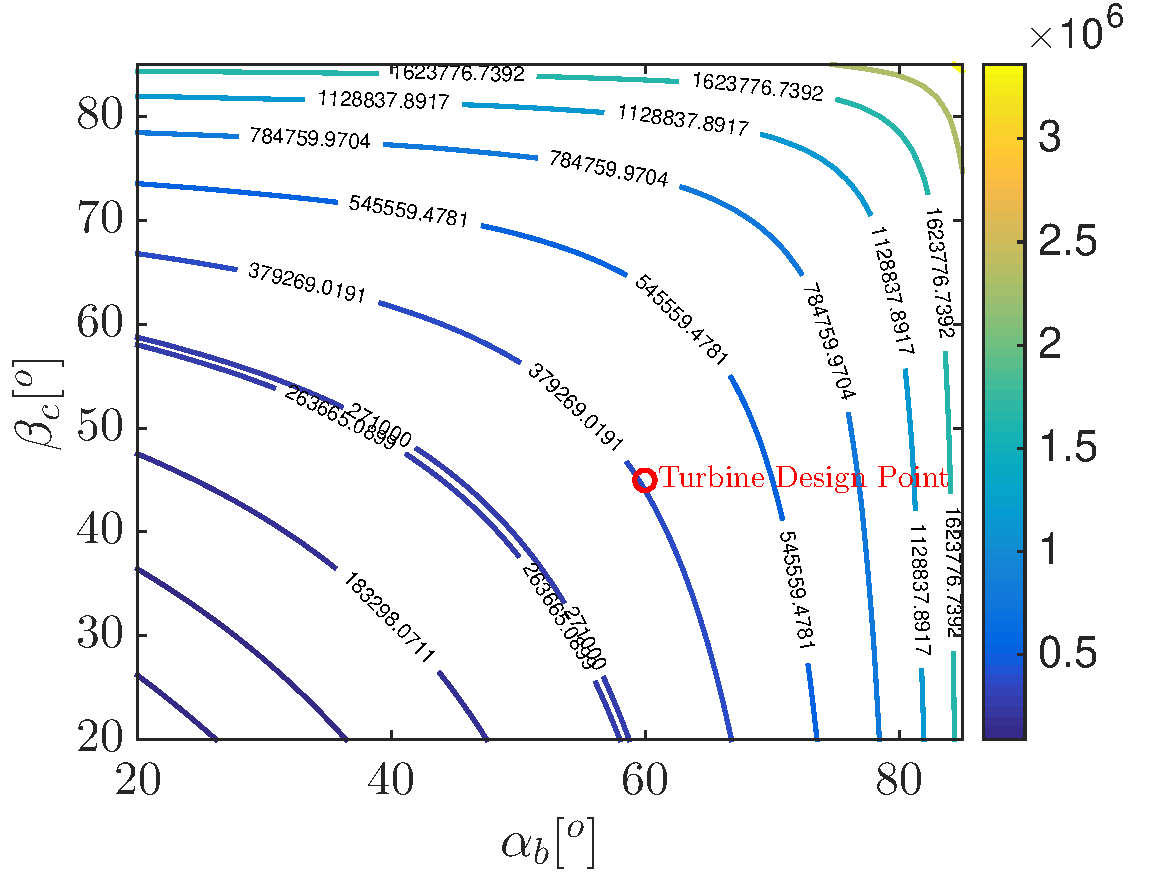
\includegraphics[width=0.6\textwidth]{p2h}
		\caption{Specific work contour.}
		\label{fig:p2h}
	\end{figure}
	
	\item[i)[5 pts]]
	From the desired work contour, it is found that the range of angles is reasonable. Theoretically, higher turning angles can be achieved in turbines compared to in compressors due to favorable pressure gradient. Therefore, flow seperation is less likely to happen in the turbine and one stage is enough for the HPT design.
	
	\item[j)[5 pts]]
	The design point of $\alpha_b = 60^\circ$ and $\beta_c = 45^\circ$ is shown in Figure~\ref{fig:p2h} by the red circle. The turbine work is higher than the target work from HPC ($2.17\times 10^5$ J/kg). Therefore, the angles proposed in the presented design is satisfactory.
	
\end{itemize}

%%%%%%%%%%%%%%%%%%%%%%%%%%%%%%%%%%%%%%%%%%%%%%%%%%%%%%%%%%%%%%%%%%%%%%%%%%%%%%%%  
\section{Part 3 Turbine Map [20 pts]}		
\begin{itemize}
	\item[a) [7 pts]]
		\begin{itemize}
			\item[(1)] Get $P_\text{t, ratio}$, $\eta_\text{t}$, $T_\text{out}$, and $W_\text{out}$ from Part 1;
			\item[(2)] Compute $M_{04}$ using Eq.~\ref{eq:u_M} as:
				\begin{equation}
					M_{04} = \left(\frac{\gamma R T_0}{u^2} - \frac{\gamma - 1}{2} \right)^{-\frac{1}{2}};
				\end{equation}
			\item[(3)] Compute $f(M_{04})$;
			\item[(4)] Compute $1/f(M_{04})$.
		\end{itemize}

	\item[b) [8 pts]]
	The initial turbine map is shown in Figure~\ref{fig:p3b}.
	\begin{figure}[H]
		\centering
		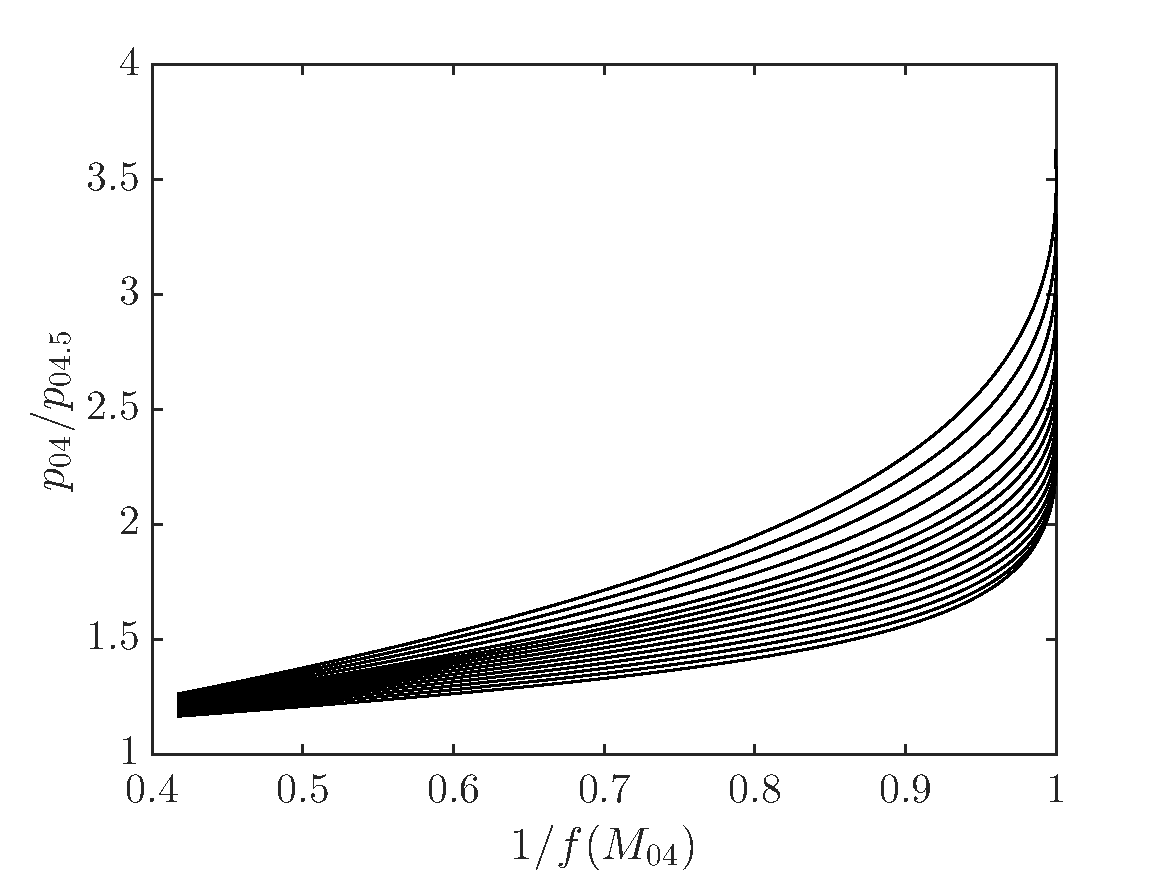
\includegraphics[width=0.6\textwidth]{p3b}
		\caption{Initial turbine map.}
		\label{fig:p3b}
	\end{figure}
	
	\item[c) [5 pts]]
	The consolidated turbine map is shown in Figure~\ref{fig:p3c}.
	\begin{figure}[H]
		\centering
		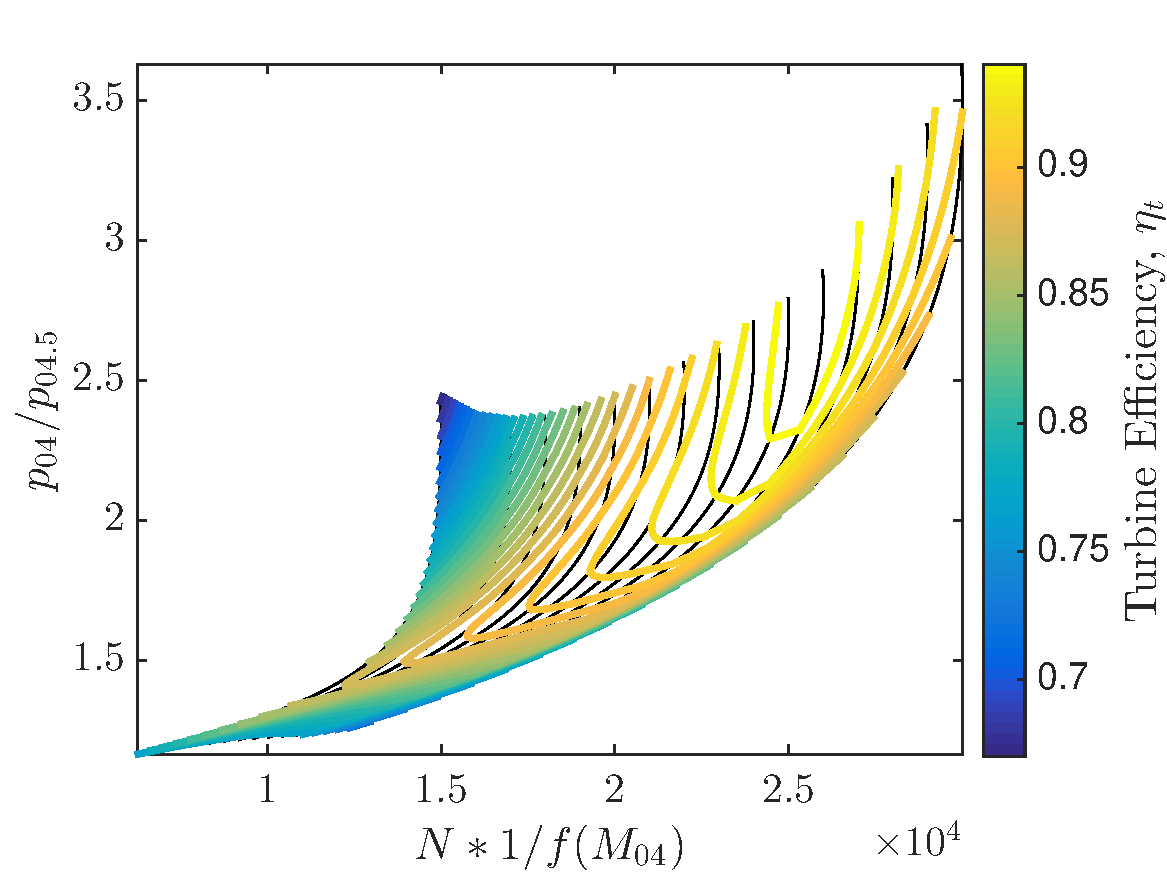
\includegraphics[width=0.6\textwidth]{p3c}
		\caption{Consolidated turbine map.}
		\label{fig:p3c}
	\end{figure}
		
\end{itemize}
%%%%%%%%%%%%%%%%%%%%%%%%%%%%%%%%%%%%%%%%%%%%%%%%%%%%%%%%%%%%%%%%%%%%%%%%%%%%%%%%
\section{Part 4 Compressor-Turbine Matching and Operating Line [30 pts]}		
\begin{itemize}
	\item[a)[7 pts]]
		\begin{itemize}
			\item[(1)] Compute the compressor map;
			\item[(2)] Compute the turbine map;
			\item[(3)] Select/guess a compressor/turbine rotating speed $N$, then get the $U$ values;
			\item[(4)] Guess an axial velocity in compressor, i.e. $u_{x,c}$;
			\item[(5)] Get pressure ratio, $f(M_{02.5})$, and the compressor work from the compressor map function which has been implemented in PSet 4;
			\item[(6)] Calculate $p_{03}$ and $p_{04}$ using the compressor pressure ratio;
			\item[(7)] Calculate the mass flow rate in the compressor, $\dot{m}_\text{compressor}$;
			\item[(8)] Equate the turbine work with the compressor work, and calculate the corresponding axial velocity in the turbine, i.e. $u_{x,t}$;
			\item[(9)] Using the chocking condition ($M_4 = 1$) to calculate the turbine inlet temperature $T_{04}$;
			\item[(10)] Get the pressure ratio and $f(M_{04})$ from the turbine map function that has been implemented in Part 3;
			\item[(11)] Calculate the mass flow rate in turbine, $\dot{m}_\text{turbine}$;
			\item[(12)] Calculate the fuel-to-mass ratio $f$;
			\item[(13)] Check if $\dot{m}_\text{compressor}(1+f)$ is equal to $\dot{m}_\text{turbine}$. If yes, go to step (3) and march to the next ratating speed $N$; if not, return to (4) and guess another axial velocity in the compressor $u_{x,c}$.
		\end{itemize}
		Note that the variable for iteration is the axial velocity in the compressor $u_{x,c}$. The objective function is the difference between $\dot{m}_\text{compressor}(1+f)$ and $\dot{m}_\text{turbine}$.
	\item[b)[8 pts] \& c)[8 pts]]
	See solution code.
		
	\item[d)[7 pts]]
	The compressor and turbine maps are shown in Figure~\ref{fig:p4d1} and~\ref{fig:p4d2} respectively. The operating line is shown by the red dashed lines one each plot.
	\begin{figure}[H]
		\centering
		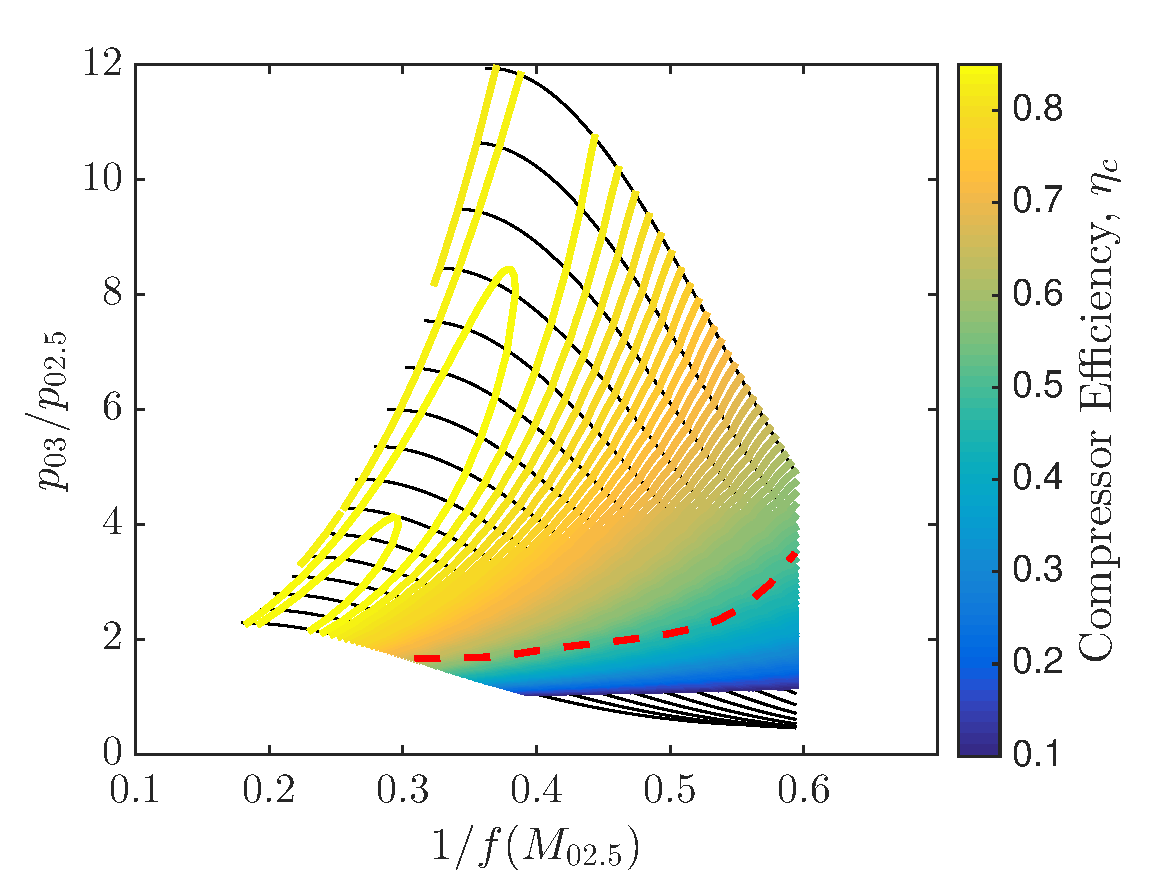
\includegraphics[width=0.6\textwidth]{p4d1}
		\caption{Compressor map.}
		\label{fig:p4d1}
	\end{figure}
		
	\begin{figure}[H]
		\centering
		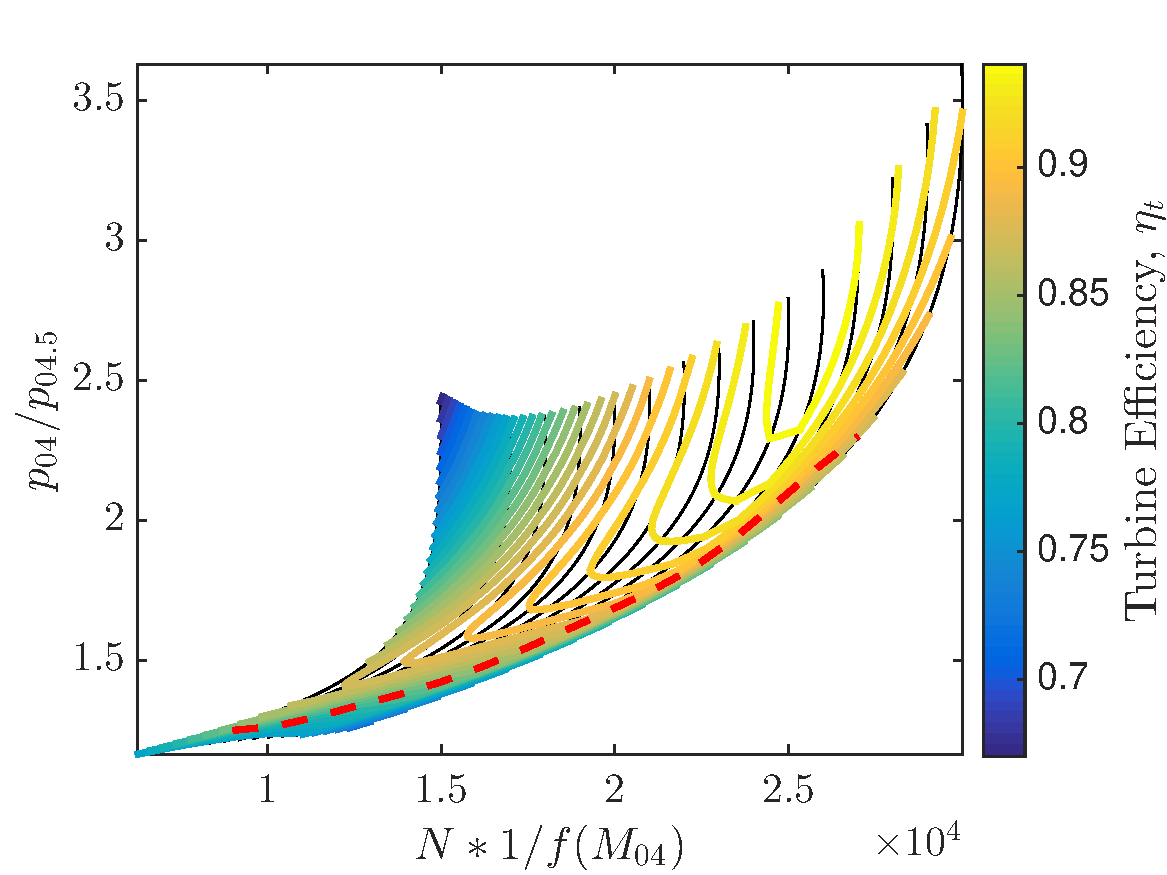
\includegraphics[width=0.6\textwidth]{p4d2}
		\caption{Turbine map.}
		\label{fig:p4d2}
	\end{figure}
	
\end{itemize}
%%%%%%%%%%%%%%%%%%%%%%%%%%%%%%%%%%%%%%%%%%%%%%%%%%%%%%%%%%%%%%%%%%%%%%%%%%%%%%%%  

\end{document}